%----------------------------------------------------------------------------
\appendix
%----------------------------------------------------------------------------
\chapter*{Appendices}\addcontentsline{toc}{chapter}{Acknowledgement}
\setcounter{chapter}{6}  % a fofejezet-szamlalo az angol ABC 6. betuje (F) lesz
\setcounter{equation}{0} % a fofejezet-szamlalo az angol ABC 6. betuje (F) lesz
\numberwithin{equation}{section}
\numberwithin{figure}{section}
\numberwithin{lstlisting}{section}
%\numberwithin{tabular}{section}

\vspace{-30px}
 \begin{figure}[h]
 \centering
 %self
 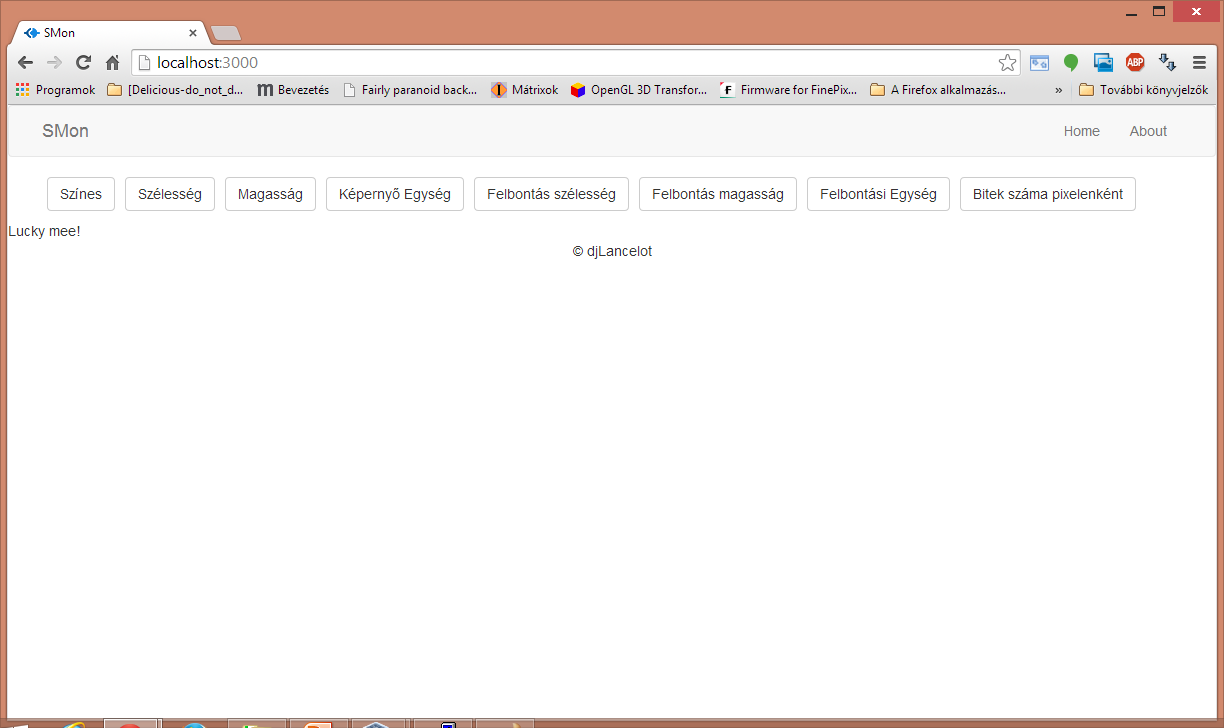
\includegraphics[width=0.6\textwidth]{figures/smon_ss.png}
 \caption{Screenshot of the test application\label{fig:smonss}}
 \end{figure}
 \begin{lstlisting}[caption={Client side JavaScript of test application\label{fig:cont}}]
 var smonApp = angular.module('smonApp',['smonSrv']);
   smonApp.controller('TestController',function($scope){
 	$scope.message = 'Lucky mee!';
   });
   smonApp.controller('formController',function($scope){
   });
 smonApp.controller('listController',['$scope','GetList',
  function($scope, List){
  	$scope.addElement=function(id, range){
  		switch(range)
  		{
  			case "http://www.w3.org/2001/XMLSchema#double":
  			case "http://www.w3.org/2001/XMLSchema#string":
  			case "http://www.w3.org/2001/XMLSchema#integer":
  				break;
  		}
  		http://www.w3.org/2001/XMLSchema#double
     	console.log(range);
     	id = '<input type="text"/>';
 	}
  	$scope.elements = List.query();
   }]);
 var smonSrv = angular.module('smonSrv', ['ngResource']);
 smonSrv.factory('GetList', ['$resource',
   function($resource){
     return $resource('/api/list', {}, {
       query: {method:'GET', isArray:true}
     });
   }]);
 
     \end{lstlisting}
 \newpage
 \begin{lstlisting}[caption={Code for the RDF parser\label{fig:rdfprs}}]
var stardog = require("stardog");
var conn = new stardog.Connection();
conn.setEndpoint("http://localhost:5820/");
conn.setCredentials("admin", "admin");
exports.index = function(req, res) {
	res.sendfile('./public/index.html'); // load the single view file (angular will handle the page changes on the front-end)
};
var getSearchables = function(callback){
	var q = "select ?property ?label ?range{?property <http://kli.uni-muenster.de/stations/hbs#filterable> true. ";
		q = q+ "?property <http://www.w3.org/2000/01/rdf-schema#label> ?label. FILTER langMatches( lang(?label), \"hu\" ) ";
		q = q + "?property <http://www.w3.org/2000/01/rdf-schema#range> ?range }"; 
	
	conn.query({ 
	        database: "smon", 
	        query: q,  
	        limit: 10, 
	        offset: 0 
	    }, callback);
	
};
exports.get_searchables = function(req, res){
	 var cb =  function (data) {
	        console.log(data.results.bindings);
	        res.json(data.results.bindings);
	};
	getSearchables(cb);  
};
exports.list_searchables = function(req, res){
	 var cb =  function (data) {
	        console.log(data.results.bindings);
	        res.render('listall', { title: 'List searchable', bindings: data.results.bindings });
	};
	getSearchables(cb);  
};
exports.list_all = function(req, res){
	conn.query({ 
	        database: "smon", 
	        query: "select distinct ?s where { ?s ?p ?o }",  
	        limit: 10, 
	        offset: 0 
	    },
	    function (data) {
	        console.log(data.results.bindings);
	        res.render('listall', { title: 'List all', bindings: data.results.bindings });
	});
  
};
 \end{lstlisting}
 
 \newpage
 
  \begin{lstlisting}[caption={Angular webpage\label{fig:angular}}]
<!DOCTYPE html>
<html ng-app="smonApp">
<head>
  <title>SMon</title>
  <link rel="stylesheet" href="https://netdna.bootstrapcdn.com/bootstrap/3.0.0/css/bootstrap.min.css" />
</head>
<!-- define angular controller -->
<body ng-controller="TestController">
  <nav class="navbar navbar-default">
    <div class="container">
      <div class="navbar-header">
        <a class="navbar-brand" href="/">SMon</a>
      </div>

      <ul class="nav navbar-nav navbar-right">
        <li><a href="#"><i class="fa fa-home"></i> Home</a></li>
        <li><a href="#about"><i class="fa fa-shield"></i> About</a></li>
      </ul>
    </div>
  </nav>
<div class="container" ng-controller="listController">
	<ul class="list-inline">
		<li ng-repeat="el in elements">
			<a href="" ng-click="addElement(el.input,el.range.value)" class="btn btn-default"> {{el.label.value}}</a> 
			<span ng-bind="el.input"></span>
		</li>
	</ul>
</div>
  <div id="main">
		<!-- this is where content will be injected -->
		{{message}}    
  </div>
  <footer class="text-center">
   &copy; djLancelot
  </footer>
    <!-- SPELLS -->
	<script src="/javascripts/angular.js"></script>
	<script src="/javascripts/angular-route.js"></script>
	<script src="/javascripts/angular-resource.js"></script>
	<script src="/javascripts/smon.js"></script>
</body>
</html>
  \end{lstlisting}